\section{\mbox{Sequentielle}~\mbox{Bifurkation}~\mbox{visueller}~\mbox{Reizrepräsentationen}}
\label{main}
\thispagestyle{plain}

Die in Abschnitt~\ref{unterschiede} vorgestellten Speziesunterschiede der
funktionalen Architektur des primären visuellen Cortex laufen auf dem
ersten Blick dem Versuch einer einheitlichen Beschreibung ihrer Entstehung
zuwider.  Es ist jedoch eine plausible Annahme, daß die Entstehung solcher
Reizrepräsentationen in den untersuchten Säugetierarten vielleicht nicht
identischen, zumindest aber verwandten Regeln folgt
(vgl. Abschn.~\ref{plastizitaet}).  Im folgenden wird aus den in
Kapitel~\ref{modell} gewonnenen Einsichten über das elastische Netz ein
allgemeines Szenarium für die Selbstorganisation visueller
Reizrepräsentationen entwickelt, mit dessen Hilfe sich die in
Kapitel~\ref{biologie}, Abschnitt~\ref{unterschiede} beschriebenen
Phänomene einheitlich beschreiben lassen.

\subsection{Vorbetrachtungen}

Von verschiedenen Autoren wurden bereits mögliche Erklärungen dieser
Speziesunterschiede vorgeschlagen.  Es ist eine plausible Annahme, daß die
Reichweite der lateralen Verbindungen zwischen den Neuronen einer
Zellschicht die Wellenlänge eines kolumnären Musters determiniert. Diese
Vorstellung resultiert aus der Überlegung, daß die Größe eines durch
einen Reiz hervorgerufenen Erregungsgebietes in einer Zellschicht mit
dieser Verbindungsreichweite verknüpft sein sollte.  Modellsimulationen
mit unterschiedlichen lateralen Verbindungsreichweiten ergeben tatsächlich
Muster unterschiedlicher Wellenlänge \cite{swindale:1992}.

Basierend auf dieser Annahme wurde zur Erklärung der verschiedenen
Wellenlängen der OD-- und OP--Systeme vorgeschlagen, daß sich jedes der
Systeme in einer eigenen neuronalen Schicht mit jeweils verschiedenen,
lateralen Verbindungsreichweiten zwischen den Neuronen ausbildet
\cite{loewel:1988}.  Die Autoren erwogen, daß nicht nur die Wellenlänge,
sondern auch die unterschiedlich ausgeprägte raümliche Ordnung der Muster
(siehe Abb.~\ref{layout} und Abb.~\ref{odcorr}) mit der Größe der
lateralen Verbindungsreichweite korreliert sein könnte. In
Modellsimulationen der koordinierten Entwicklung von OD-- und OP--Karten
bedarf es jedoch zusätzlicher Annahmen, um die beobachtete Anisotropie der
OD--Karte im Affen zu reproduzieren \cite{swindale:1992}.  Eine räumliche
Trennung der Muster verschiedener Wellenlänge erschwert außerdem die
Erklärung der lokalen geometrischen Beziehung zwischen den Mustern der
Okulardominanz und der Orientierungspräferenz, wie sie im visuellen Cortex
von Affen und Katzen beobachtet wird (vgl. Abschn.~\ref{90grad}).

In biologischen Systemen hängt die Größe eines lokalen Erregungsgebietes
in einer bestimmten Zellschicht mindestens von zwei Faktoren ab: Der
Reichweite der lateralen Verbindungen der Neurone innerhalb einer
Zellschicht und der Ausdehnung der im primären visuellen Cortex
terminierenden Axonenäste.  Diese Axonenäste stehen am Ende der
Nervenbahn (\emph{radiatio optica}, vgl. Abschn.~\ref{sehbahnkap}), die das
LGN mit dem Cortex verbindet.  Es gibt experimentelle Evidenz dafür, daß
beide Größen, sowohl die laterale Verbindungsreichweite als auch die
Ausdehnung der im Cortex terminierenden Axonenäste, im Laufe der ersten
Lebenswochen abnehmen. Evidenz für abnehmende laterale
Verbindungsreichweiten lieferten u.A. Untersuchungen am Frettchen
\cite{katz:1994}\footnote{Die Autoren dieser Arbeit diskutieren hauptsächlich
die Vergrößerung der langreichweitigen Verbindungen der Neurone. Jedoch
ist aus den Daten ersichtlich, daß die lokale Verbindungsreichweite im
Laufe der Entwicklung abnimmt.}. Kleine und große Axonenäste in jungen und
adulten Katzen wurden von \citeasnoun{ferster:1978}
bzw. \citeasnoun{levay:1979} beobachtet.  Es ist also plausibel anzunehmen,
daß die Ausdehnung eines typischen Erregungsgebietes im visuellen Cortex
im Laufe der Entwicklung abnimmt. Diese Annahme und das kritische Verhalten
des elastischen Netzes sind wichtige Vorraussetzungen für das im folgenden
Abschnitt entwickelte Szenarium.
\setcounter{footnote}{1}

\subsection{Das sequentielle Bifurkationsszenarium}

\begin{figure}[t]
\centering
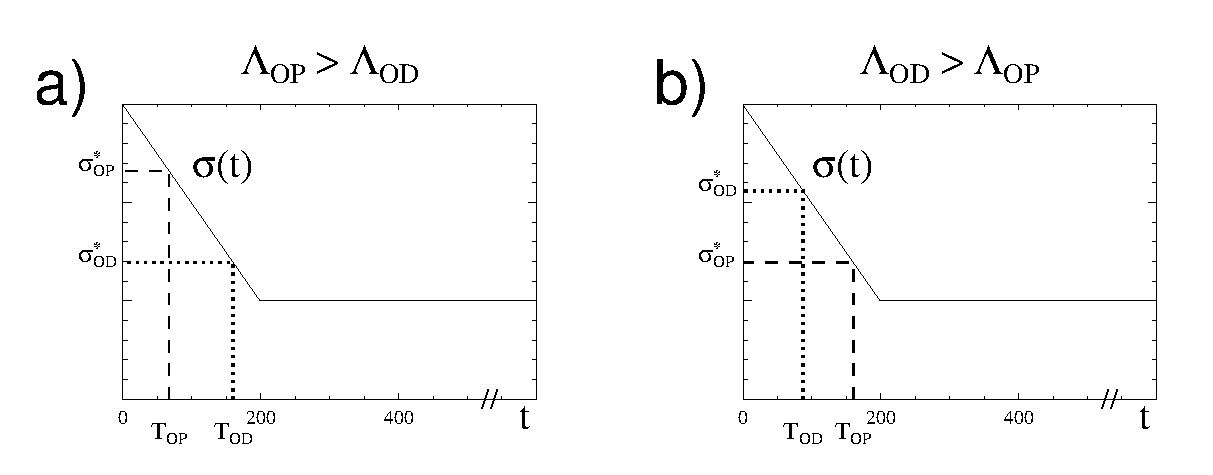
\epsfig{file=pics/seqbif.eps,width=\textwidth}
\caption{Skizze der in den Simulationen zur koordinierten Enstehung von
OD-- und OP--Mustern verwendeten Zeitentwicklung des
Modell--Parameters~$\sigma$ \textbf{a)} ``Katzen--ähnliche'' Simulation:
Hier entsteht die Orientierungspräferenz zuerst, und hat daher die
größere Wellenlänge. \textbf{b)} ``Affen--ähnliche'' Simulation: in
diesem Fall ensteht das Muster der Okulardominanz zuerst (und hat daher die
größere Wellenlänge).}
\label{zeitentwicklung}
\end{figure}

Wie in Kapitel~\ref{modell} dargestellt, existiert im elastischen Netz für
jede emergierende kolumnäre Struktur eine unabhängige, kritische
Kooperationsreichweite $\sigma_i^\ast$.  Diese wiederum wird durch die
Stimulusvarianz  in der entsprechenden Merkmalsraumdimension bestimmt. Die
kritischen Kooperationsreichweiten für die Muster der
Orientierungspräferenz und die Okulardominanz werden also in der Regel
verschiedene Werte annehmen. Qualitativ sind dabei zwei Fälle zu
unterscheiden:

\begin{enumerate}
\item $\sigma_{\text{OD}}^\ast > \sigma_{\text{OP}}^\ast$
\item $\sigma_{\text{OD}}^\ast < \sigma_{\text{OP}}^\ast$
\end{enumerate}

Vor diesem Hintergrund hat die Annahme einer zeitabhängigen, während der
Entwicklung kontinuierlich schrumpfenden Kooperationsreichweite $\sigma(t)$
folgende Konsequenzen für die Simulation der Dynamik~\eqref{endyn}: Ein
kontinuierlich abnehmendes $\sigma(t)$ unterschreitet die verschiedenen,
kritischen Kooperationsreichweiten $\sigma_i^\ast$ der
kolumnären Muster \emph{sequentiell}. Zu jedem Zeitpunkt $t$, an dem
$\sigma(t)$ eine dieser kritischen Reichweiten $\sigma_i^\ast$
unterschreitet, wird die homogene Lösung in der entsprechenden Dimension
instabil; es bilden sich kolumnäre Muster mit einer durch das jeweilige
$\sigma_i^\ast$ determinierten Wellenlänge.  Die unterschiedlichen
Längenskalen verschiedener kolumnärer Systeme werden also in eine
\emph{zeitliche Abfolge von Instabilitäten} übersetzt. Dies bezeichnen
wir als \emph{sequentielles Bifurkationsszenarium}.  Den beiden oben
angeführten Verhältnissen von $\sigma_{\text{OD}}^{\phantom{\ast}}$ zu
$\sigma_{\text{OP}}^{\phantom{\ast}}$ entspricht damit (1.)
$\Lambda_{\text{OD}} > \Lambda_{\text{OP}}$ und (2.) $\Lambda_{\text{OD}} <
\Lambda_{\text{OP}}$.

Die in Affen und Katzen beobachteten, unterschiedlichen
Wellenlängenverhältnisse lassen sich mit dem sequentiellen
Bifurkationsszenarium also auf elegante Weise einheitlich erklären: Das
sequentielle Bifurkationsszenarium sagt voraus, daß sich in jeder Spezies
das Muster mit der größeren Wellenlänge zuerst ausbildet
(vgl. Abb.~\ref{zeitentwicklung}). In Modellsimulation zum Szenarium
werden die genauen Wellenlängenverhältnisse notwendigerweise
reproduziert.  Inwieweit die Annahme einer unterschiedlichen
Entstehungsreihenfolge der OD-- und OP--Karten auch die räumliche Ordnung
dieser Karten erklären kann, wird in den folgenden Abschnitten untersucht.

\subsection{Dynamische Umordnung der Okulardominanz}
\label{odord}

Das Muster der Okulardominanz im Affen zeigt einen hohen Grad räumlicher
Kohärenz (vgl. Abschn.~\ref{unterschiede}): Die OD--Domänen bilden ein
System paralleler Streifen, die selten verzweigen und hauptsächlich
senkrecht zum Arealrand verlaufen \citeaffixed{levayetal:1985}{siehe
z.B.}. Um diese Ordnung des Musters zu quantifizieren wurde die
Autokorrelation

\begin{small}
\begin{equation}
C(\mathbf{r})=\left<\left(O(\mathbf{x+r})-\bar{O}\right)\ast\left(O(\mathbf{x})-\bar{O}\right)\right>_{\mathbf{x}\,\in\,\text{Bild}},\;\;\bar{O}=\left<O(\mathbf{x})\right>_{\mathbf{x}\,\in\,\text{Bild}}
\label{autocorr}
\end{equation}
\end{small}

\noindent digitalisierter OD--Karten von Affen, strabismischen und
normalsichtigen Katzten berechnet.  Im gezeigten Ausschnitt aus der
OD--Karte des Affen sieht man die globale Vorzugsrichtung der Domänen
eutlich.  Dieser Augenschein wird durch die einige Perioden anhaltende
Modulation der Autokorrelation bestätigt (siehe Abb.~\ref{odcorr}).
Dagegen zerfällt die Autokorrelation sowohl der OD--Karte der
strabismischen als auch der normalsichtigen Katze in allen Richtungen
schnell. Die Domänen dieser beiden Muster zeigen keine detektierbare
Vorzugsrichtung\footnote{Interessanterweise ist die Monokularität der
Zellen in A17 strabismischer Katzen stärker ausgeprägt als in V1 des
Affen (vgl. Abschn.~\ref{unterschiede}, Abb.~\ref{okuhist}).  Also läßt
sich weder der Grad der Monokularität der Neurone noch die Reichweite
ihrer lateralen Verbindungen zur Erklärung der unterschiedlichen
Anisotropie der OD--Muster in Katzen und Affen heranziehen.}.
\setcounter{footnote}{1}

\begin{figure}[h!]
\centering
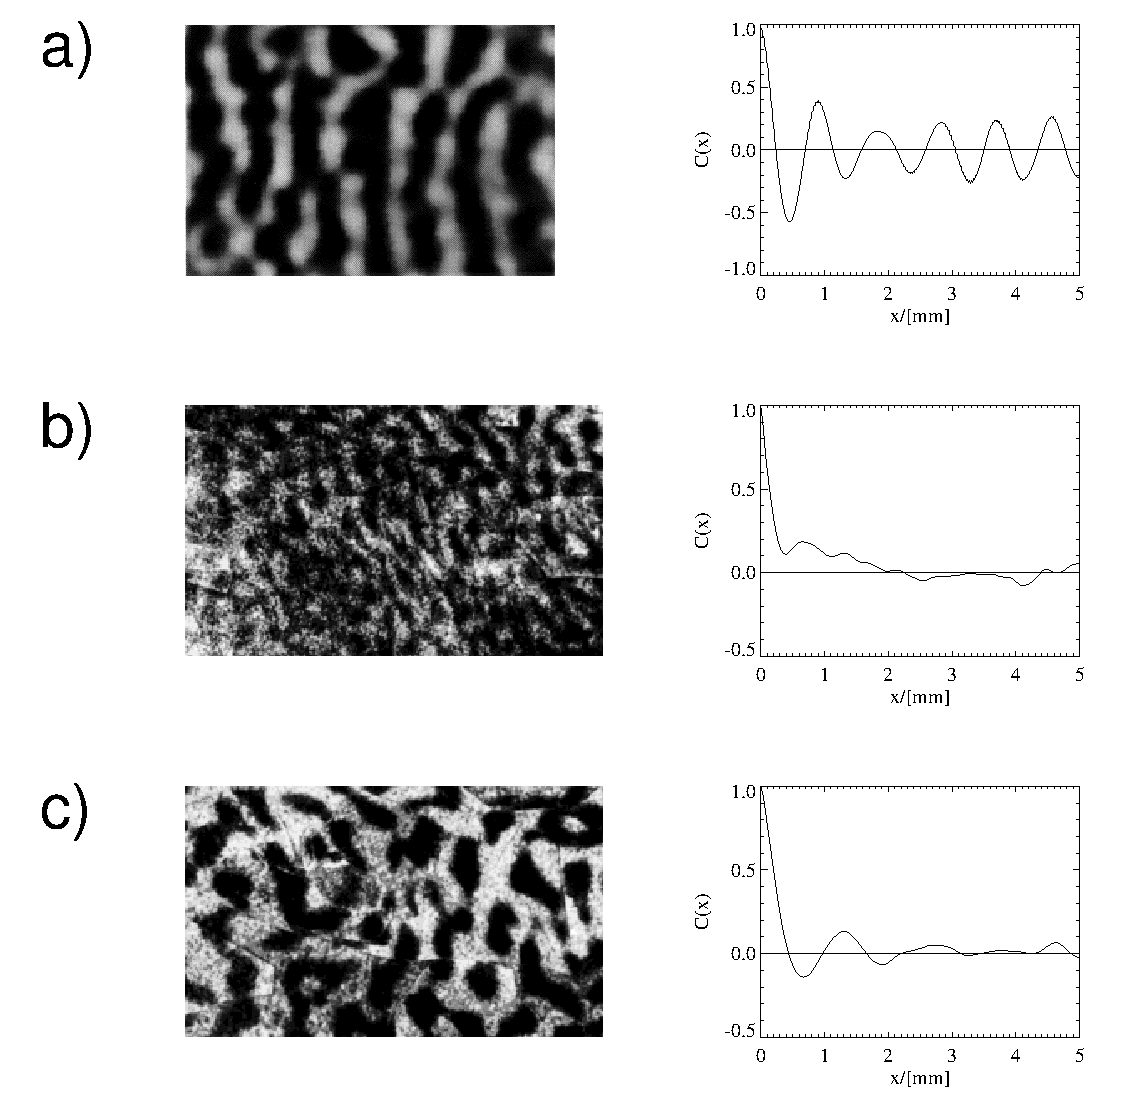
\epsfig{file=pics/od_corr.eps,width=11.9cm}
\caption{Die Bilder zeigen typische Auschnitte des OD--Musters aus V1 eines
Affen \protect\citeaffixed{grinvald:1991}{6.4mm$\times$4.3mm, optisches
Ableiten,} und aus A17 einer normalsichtigen und strabismischen Katze
\protect\citeaffixed{loewel:1987}{jeweils 5mm$\times$3mm, [$^3$H]--Prolin
Markierung,}. Neben jedem Bild ist die dazugehörige Autokorrelation
$C(\mathbf{r})\vert_{\mathbf{r}={\binom{x}{0}}}$ gezeigt.}
\label{odcorr}
\end{figure}

Die in Simulationen aufgrund der Isotropie der Dynamik
hervorgebrachten Strukturen sind notwendigerweise statistisch isotrop
(siehe Abschn.~\ref{stabilitaet}).  Der ersten Etablierung eines solchen
Musters durch einen linearen Instabilitätsmechanismus kann jedoch
eine Phase der kontinuierlichen, nichtlinearen Umordnung folgen.  Simulationen der Entstehung von Okulardominanzkarten mit
dem elastischen Netz~\eqref{endyn} zeigen, daß das Muster tatsächlich in
dieser nichtlinearen Umordnungsphase anisotrop wird und sich in ein System
paralleler Streifen umordnet (siehe Skizze in
Abb.~\ref{umordnung}).

\subsection{Ergebnisse numerischer Simulationen zum Szenarium}
\label{numerg}

Zur Erzeugung kolumnärer Strukturen die sich durch das sequentielle
Bifurkationsszenarium ergeben wurde die Dynamik~\eqref{endyn} ausgehend vom
Anfangszustand $\mathbf{R}_0(\mathbf{x}) = (x,\, y,\, 0,\, 0,\, 0) $ für
ein endliches Cortexareal $\cal T$ mit periodischen Randbedingungen
numerisch integriert (für Details dazu siehe Anhang~\ref{anhang2}).

In einer Reihe von  Simulation  wurden die Stimulusvarianzen in den
Merkmalsdimensionen der Orientierungspräferenz und Okulardominanz  so
eingestellt, daß nicht nur $\sigma^\ast_{\text{OP}}>\sigma^\ast_{\text{OD}}$
(und damit $\Lambda_{\text{OP}} > \Lambda_{\text{OD}}$,
vgl. Abb.~\ref{zeitentwicklung}a), sondern auch
das aus A17 der Katze bekannte Verhältnis der Wellenlängen beider
Muster (vgl.~Abschn.~\ref{unterschiede}, Abb.~\ref{wavelength})
erhalten wurde.  In Simulationen mit kontinuierlich schrumpfenden
$\sigma(t)$ entsteht dann das Muster der Orientierungspräferenz vor dem
Muster der Okulardominanz (siehe Abb.~\ref{opod}).

\begin{figure}[h!]
\centering
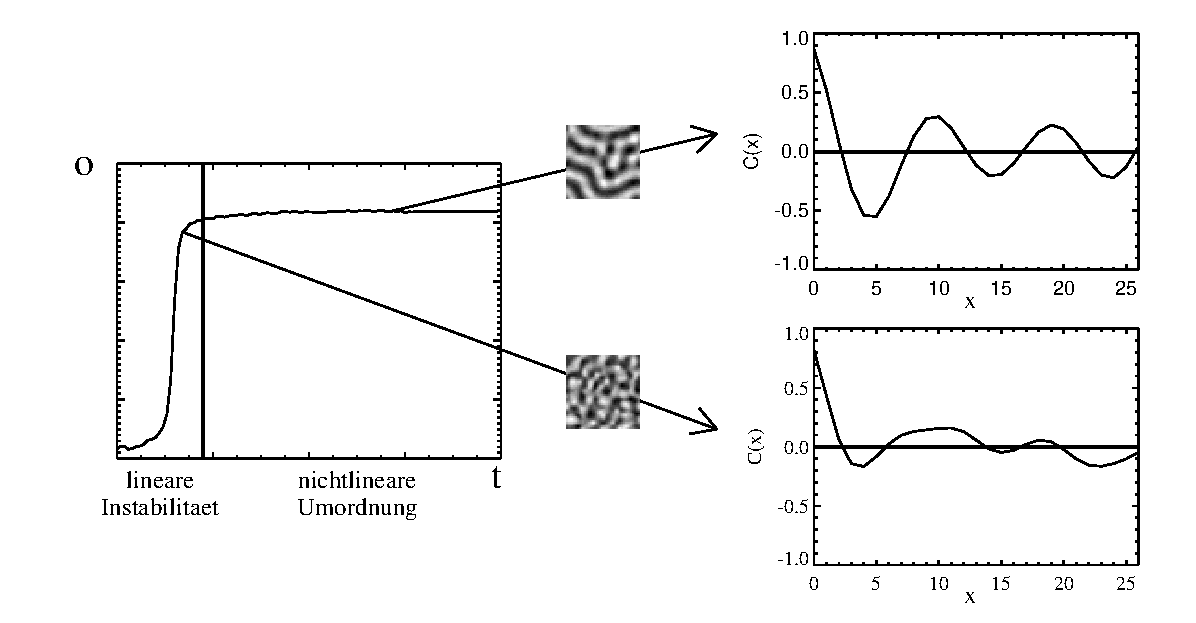
\epsfig{file=pics/umordnung.eps,width=\textwidth}
\caption{Simulation der Okulardominanz mit dem elastischen Netz. Links:
typische Entwicklung der Amplitude der instabilen Lösung. Rechts:
Autokorrelation eines typischen OD--Musters kurz und lange nach der
Instabilität.}
\label{umordnung}
\end{figure}


\begin{figure}[p]
\centering
\begin{sideways}
\epsfig{file=pics/opod_rot.eps,height=\textwidth}
\end{sideways}
\caption{Momentaufnahmen der koordinierten Entwicklung von Okular\-do\-minanz--
und Orientierungskarten für
$\sigma^\ast_{\text{OP}}>\sigma^\ast_{\text{OD}}$ (Szenarium
Abb.~\ref{zeitentwicklung}a). Die Farb--/Grauwertintensität spiegelt
die Amplitude der Strukturen wieder ($40\times 40$ Neurone mit periodischen
Randbedingungen, $\eta_{\text{rel}}=0.0025$,
$\sigma^\ast_{\text{OD}}=0.0837$, $\sigma^\ast_{\text{OP}}=0.1189$
$\Longrightarrow$ $\Lambda_{\text{OD}}/\Lambda_{\text{OP}}=4/5$).}
\label{opod}

\begin{center}
\begin{sideways}
\epsfig{file=pics/odop_rot.eps,height=\textwidth}
\end{sideways}
\end{center}
\caption{Momentaufnahmen wie oben, jedoch in einer Simulation mit
$\sigma^\ast_{\text{OD}}>\sigma^\ast_{\text{OP}}$, ensprechend des Szenariums in
Abb.~\ref{zeitentwicklung}b ($40\times 40$ Neurone mit
periodischen Randbedingungen, $\eta_{\text{rel}}= 0.0025$,
$\sigma^\ast_{\text{OD}}=0.0976$, $\sigma^\ast_{\text{OP}}=0.0679$
$\Longrightarrow$ $\Lambda_{\text{OD}}/\Lambda_{\text{OP}}=6/5$).}
\label{odop}
\end{figure}

In einer weiteren Reihe von Simulationen wurde die zweite Variante des
Szenariums (Abb.~\ref{zeitentwicklung}b) untersucht: Die Varianzen der
Reizverteilungen in den Merkmalsdimensionen wurden entsprechend des für
den Affen geltenden Wellen\-längen\-ver\-hältnisses gewählt. Da hier
$\Lambda_{\text{OD}} > \Lambda_{\text{OP}}$ ist, entsteht in Simulationen
mit kontinuierlich schrumpfenden~$\sigma(t)$ also das Muster der
Okulardominanz vor dem Muster der Orientierungspräferenz (siehe
Abb.~\ref{odop}).

Abbildung~\ref{simres} stellt die Endkonfigurationen der in den
Abbildungen~\ref{opod} und \ref{odop} gezeigten, typischen
Simulationsergebnisse zu diesem Szenarium nocheinmal vergleichend vor.  Im
einen Fall (Abb.~\ref{opod} und Abb.~\ref{simres}, links) bildet die
Okulardominanz perlige Domänen. Die Grenzlinien dieser Domänen verlaufen
dabei oft geschlossen um die Singularitäten der Orientierungskarte.  Im
anderen Fall bildet das Muster der Okulardominanz ein System ausgedehnter
Streifen, die selten verzweigen und über weite Abschnitte parallel
verlaufen (Abb.~\ref{odop} und Abb.~\ref{simres}, rechts).
In beiden Fällen des Szenariums stimmen die Ergebnisse aller durchgeführten
Simulationen gut mit den experimentell beobachteten Karten überein. Das
nicht nur die Wellenlängenverhältnisse sondern, wie in Abb.~\ref{simres}
gezeigt, auch die unterschiedlichen Layouts der Muster korrekt reproduziert
werden, bedarf einer zusätzlichen Erklärung.

\begin{figure}[t]
\centering
\begin{minipage}[t]{6.2cm}
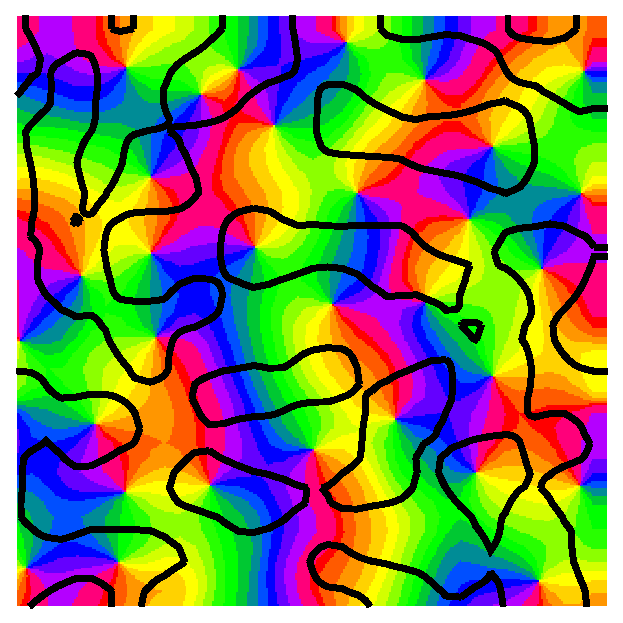
\epsfig{file=pics/op+od.eps,width=6.2cm}
\end{minipage}
\hskip0.4cm
\begin{minipage}[t]{6.2cm}
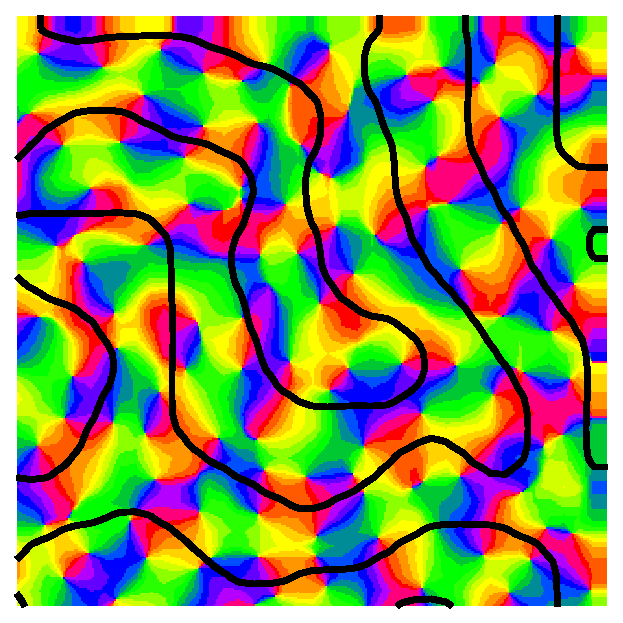
\epsfig{file=pics/od+op.eps,width=6.2cm}
\end{minipage}
\caption{Vorhersage des funktionalen Layouts von Okulardominanz-- und
Orientierungspräferenz--Karten für die Katze (links, Ergebnis der in
Abb.~\ref{opod} gezeigten Simulation) und den Affen (rechts, Ergebnis der
in Abb.~\ref{odop} gezeigten Simulation).  Die Abbildungen zeigen eine
Überlagerung der Iso--Orientierungsdomänen (farbig) mit den Grenzenlinien
der Okulardominanzkolumnen (schwarz).}
\label{simres}
\end{figure}

\begin{figure}[p]
\centering
\begin{sideways}
\epsfig{file=pics/oddev.eps,height=12cm}
\end{sideways}
\caption{Momentaufnahmen der Weiterentwicklung einer Okulardominanzkarte.
Die am Anfang gezeigte Karte entstand in einer typischen Simulation mit
$\sigma^\ast_{\text{OP}}>\sigma^\ast_{\text{OD}}$. Ihre Weiterentwicklung in
dieser Simulation zeigt die untere Reihe. Die obere Reihe zeigt die
Weiterentwicklung der Karte \emph{ohne} das Muster der
Orientierungspräferenz (beide Reihen: $40\times 40$ Neurone,
$\sigma(t)=\sigma^\ast_{\text{OD}}*0.9$, $\eta_{\text{rel}}=0.001$).}
\label{oddev}

\begin{center}
\begin{sideways}
\epsfig{file=pics/angledev.eps,width=9cm}
\end{sideways}
\end{center}
\caption{Typische Entwicklung der geometrischen Beziehung zwischen den
Iso--Orientierungslinien und den Okulardominanz--Grenzlinien im Anschluß
an die primäre Etablierung beider Strukturen.}
\label{angledev}
\end{figure}

Die Wechselwirkung der verschiedenen kolumnären Strukturen im elastischen
Netz führt zu einer Reproduktion der in Abschnitt~\ref{90grad}
vorgestellten, geometrischen Beziehung zwischen den
Iso--Orientierungslinien und den Grenzlinien der Okulardominanz
(vgl. \citeasnoun{erwin:1995} und Abb.~\ref{odop_hist}, links). Daher
erschient die Annahme plausibel, daß auch im visuellen Cortex von Katzen
und Affen diese geometrische Beziehung Ergebnis einer dynamischen
Interaktion der OD-- und OP--Karten ist. In diesem Fall wäre das Muster
der Okulardominanz in der Katze ``versklavt'': Die früher entstandene
Orientierungskarte würde die Umorganisation der Okulardominanz in ein
System parallerel Bänder mit Vorzugsrichtung verhindern.  Durch die
Wechselwirkung beider Muster im Modell bildet sich in diesem Fall die
später entstehende Okulardominanzkarte so aus, daß ihre Grenzlinien
häufig geschlossene Kurven um Pinwheels bilden. Dies erfüllt die
Randbedingung der in Abschnitt~\ref{90grad} vorgestellten, geometrischen
Beziehung beider Strukturen.

Um diese Hypothese der Versklavung der Okulardominanz zu testen, wurde nach
der Entstehung beider Muster in Simulationen mit
$\sigma^\ast_{\text{OP}}>\sigma^\ast_{\text{OD}}$ untersucht, wie sich die
Okulardominanzkarte \emph{mit} bzw. in Abwesenheit der Orientierungskarte
weiterentwickelt. Wie Abbildung~\ref{oddev} an einem Beispiel zeigt, ordnet
sich der identische Ausgangszustand der Okulardominanzkarte ohne
Orientierungskarte in ein System paralleler Bänder mit Vorzugsrichtung um.
Unter Brücksichtigung der Randbedingung stumpfer Schnittwinkel zwischen
Iso--Orientierungslinien und Okulardominanz--Grenzlinien läßt sich also
in der Katze das Layout der Muster durch ihre sequentielle Enstehung
erklären.  Ein wie im Affen beobachtetes, räumlich kohärentes Muster der
Okulardominanz dagegen kann ebenfalls nur durch dynamische Umordnung in
Abwesenheit des Musters der Orientierungspräferenz entstehen
(vgl. Abschn.~\ref{odord}).  Aus unseren Simulationen folgt also, daß die
Wechselwirkung der Strukturen ihr Erscheinungsbild entscheidend
beeinflußt.

Berechnet man, wie in Abschnitt~\ref{90grad} dargelegt, die Verteilung der
Schnittwinkel zwischen den Iso--Orientierungslinien und den Grenzlinien der
Okulardominanz für mehrere Konfigurationen im Zuge der Entwicklung, so
zeigt sich, das diese geometrische Beziehung beider Muster im Modell erst
in einem Zeitraum nach der primären Etablierung der Muster realisiert
wird (ein Beispiel dafür zeigt Abb.~\ref{angledev}).  Dies wird in allen
durchgeführten Simulationen der koordinierten Entwicklung von OD-- und
OP--Karten ungeachtet ihrer Entstehungsreihenfolge beobachtet und zeigt,
daß diese geometrische Beziehung beider Muster Resultat eines dynamischen
Umordnungsprozess in der nichtlinearen Phase der Entwicklung ist.
